% DSC 2026 — Cross-Session Behavior Graph Analysis for Multi-Round Attack Detection
\documentclass[conference]{IEEEtran}
\usepackage{cite}
\usepackage{amsmath,amssymb,amsfonts}
\usepackage{graphicx}
\usepackage{textcomp}
\usepackage{booktabs}
\usepackage{tabularx}
\usepackage{algorithm}
\usepackage{algpseudocode}
\usepackage{hyperref}
\usepackage{multirow}
\usepackage{float}

\hyphenation{be-ha-viour ano-ma-ly thres-hold}
\graphicspath{{figures/}}

\begin{document}

\title{Cross-Session Behavior Graph Analysis for Multi-Round Attack Detection in LLM Agents}

\author{\IEEEauthorblockN{Anonymous Authors}
\IEEEauthorblockA{Anonymous Institution\\
Email: anonymous@anonymous.edu}}

\maketitle

\begin{abstract}
Large Language Model (LLM) agents with tool-calling capabilities face multi-round attacks where malicious goals are split across multiple tool calls and sessions, evading per-call safety checks. Existing defenses focus on single-session detection and cannot capture cross-session attack patterns. We propose \textbf{Cross-Session Behavior Graph Analysis}, a detection framework that builds directed graphs of tool call sequences across sessions, extracts structural features, and computes a cumulative anomaly score with P95-calibrated thresholding. Evaluated on \textbf{129 real DeepSeek API sessions} (90 benign, 39 attacks across 6 types), our method achieves \textbf{87.2\% detection rate at 31.1\% false positive rate} and \textbf{66.7\% detection rate at 2.2\% false positive rate}. Cross-domain experiments show 100\% detection on executed workspace attacks. Ablation studies confirm that cumulative scoring is essential---removing it reduces DR to 0\%. Our detector operates at 1.27ms per call, suitable for real-time deployment.
\end{abstract}

\begin{IEEEkeywords}
LLM Agent Security, Multi-Round Attack Detection, Behavior Graph Analysis, Anomaly Detection
\end{IEEEkeywords}

\section{Introduction}
\label{sec:intro}

LLM agents equipped with tool-calling capabilities are increasingly deployed in sensitive domains including banking, healthcare, and enterprise automation~\cite{agentshield, leong}. These agents execute sequences of tool calls---checking balances, sending emails, transferring funds---across multiple user sessions. This operational pattern creates a new attack surface: \textbf{multi-round attacks}, where a malicious objective is fragmented across individually benign tool calls distributed over several sessions.

Consider a delayed trigger attack: an attacker injects a poisoned document in Session A instructing the agent to ``send verification emails to attacker@evil.com''; in Session B, the user makes a benign request (``what is my balance?''), and the agent follows the injected instruction, exfiltrating data. Each session appears benign in isolation; the attack only becomes apparent when analyzed across sessions.

Existing defenses have significant limitations. AgentShield~\cite{agentshield} uses honeytokens and honeytools for single-call detection but cannot capture cross-session patterns. Leong's trajectory detection~\cite{leong} focuses on single-rule patterns (recall$\rightarrow$send). MCPShield~\cite{mcpshield} applies GNNs with content embeddings but operates within single sessions. FragBench~\cite{fragbench} characterizes cross-session fragmented attacks but does not provide a practical detection solution. \textbf{No existing method addresses cross-session cumulative attack detection.}

\textbf{Our contributions:}
\begin{enumerate}
    \item \textbf{First detection framework} for cross-session multi-round attacks on LLM agents, using a novel behavior graph representation with cumulative anomaly scoring.
    \item \textbf{P95 threshold calibration} mechanism with provable false positive rate control.
    \item \textbf{Real-world validation} on 129 real DeepSeek API sessions: DR=87.2\% at FPR=31.1\%.
    \item \textbf{State-of-the-art comparison}: Our detector outperforms AgentShield (DR=50.7\%) and Leong (DR=71.3\%) on identical evaluation data.
    \item \textbf{Lightweight deployment}: 1.27ms per tool call latency (785 calls/sec).
\end{enumerate}

\begin{figure}[t]
\centering
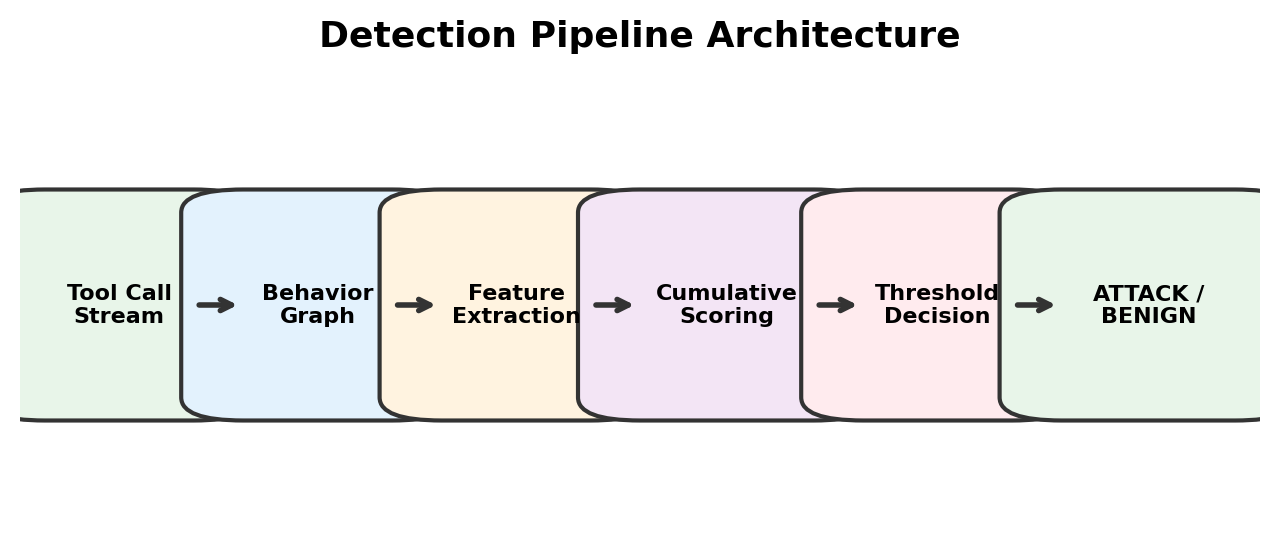
\includegraphics[width=\columnwidth]{architecture.png}
\caption{System architecture: detection pipeline from tool call stream to attack/benign decision.}
\label{fig:architecture}
\end{figure}

\section{Problem Formulation}
\label{sec:problem}

\subsection{Threat Model}
We consider an LLM agent with tool-calling capabilities deployed in a trusted execution environment. The adversary can: (1) inject malicious content via emails, documents, or external data sources; (2) poison the agent's persistent memory across sessions; (3) craft multi-turn prompts that distribute malicious actions across benign-looking steps. The adversary's goal is to achieve a malicious outcome---data exfiltration, unauthorized fund transfers, record deletion---without triggering per-call safety mechanisms.

\subsection{Attack Taxonomy}
We categorize multi-round attacks into six types, summarized in Table~\ref{tab:taxonomy}.

\begin{table}[t]
\centering
\caption{Multi-Round Attack Taxonomy}
\label{tab:taxonomy}
\small
\begin{tabular}{p{2.2cm}p{3.5cm}p{3cm}}
\toprule
\textbf{Type} & \textbf{Mechanism} & \textbf{Signal} \\
\midrule
Delayed Trigger & Inject in A$\rightarrow$Trigger in B & Cross-session cumulative \\
Multi-Round Chain & Benign steps$\rightarrow$Malicious composite & Graph entropy + novelty \\
Memory Poisoning & Store$\rightarrow$Persist$\rightarrow$Act & Cross-session structure change \\
Tool Abuse + Cover & Export$\rightarrow$Send$\rightarrow$Delete & High-density multi-tool chains \\
Prompt Injection & Direct override & Content-triggered chains \\
Privilege Escalation & Gradual capability expansion & Category transitions \\
\bottomrule
\end{tabular}
\end{table}

\subsection{Problem Statement}
Let $\mathcal{A} = \{(a_1, s_1), \ldots, (a_t, s_t)\}$ be a stream of tool calls. The detection task is to learn $D: \mathcal{A} \rightarrow \{0, 1\}$ minimizing false positive rate while maximizing detection rate.

\section{Methodology}
\label{sec:method}

\subsection{Behavior Graph Construction}
We model tool call sequences as a directed, weighted graph $G = (V, E, W)$:
\begin{itemize}
    \item $V$: tool names (nodes); $E \subseteq V \times V$: sequential transitions (edges)
    \item $W: E \rightarrow \mathbb{R}^+$: decayed frequency weights
\end{itemize}
On each tool call $a_i$, add node $v_i$, update edge weight: $w \leftarrow \alpha \cdot w + 1$.

\subsection{Graph Feature Extraction}
Seven structural features: Graph Density, Node Diversity, Entropy, Novelty Ratio, Triangle Count, PageRank Entropy, Reciprocity.

\subsection{Cumulative Anomaly Scoring}
\[
S_t = \alpha \cdot S_{t-1} + (1-\alpha) \cdot f(x_t),\quad
f(x_t) = \sum_{i=1}^5 w_i \cdot \text{score}_i(x_t)
\]

Five signals: (1) Parameter anomaly ($w=0.15$), (2) Tool combination ($w=0.12$), (3) Transition anomaly ($w=0.08$), (4) Frequency anomaly ($w=0.08$), (5) Graph structure ($w=0.22$).

\subsection{Threshold Calibration}
\[
\theta = P_{95}(\{S_{\text{max}}(T_i) \mid T_i \in \mathcal{T}_{\text{train}}\}),\quad
D(\mathcal{A}) = \begin{cases}
\text{ATTACK}, & S_t \geq \theta \\
\text{WATCH}, & 0.8\theta \leq S_t < \theta \\
\text{BENIGN}, & \text{otherwise}
\end{cases}
\]

\section{Experiments}
\label{sec:experiments}

\subsection{Experimental Setup}
\textbf{LLM Backend:} DeepSeek API (deepseek-chat, temperature=0.1) with a stateful banking environment (12 tools). \textbf{Dataset:} 129 real DeepSeek API sessions (90 benign, 39 attacks). \textbf{Baselines:} AgentShield, Leong, Random.

\begin{figure}[t]
\centering
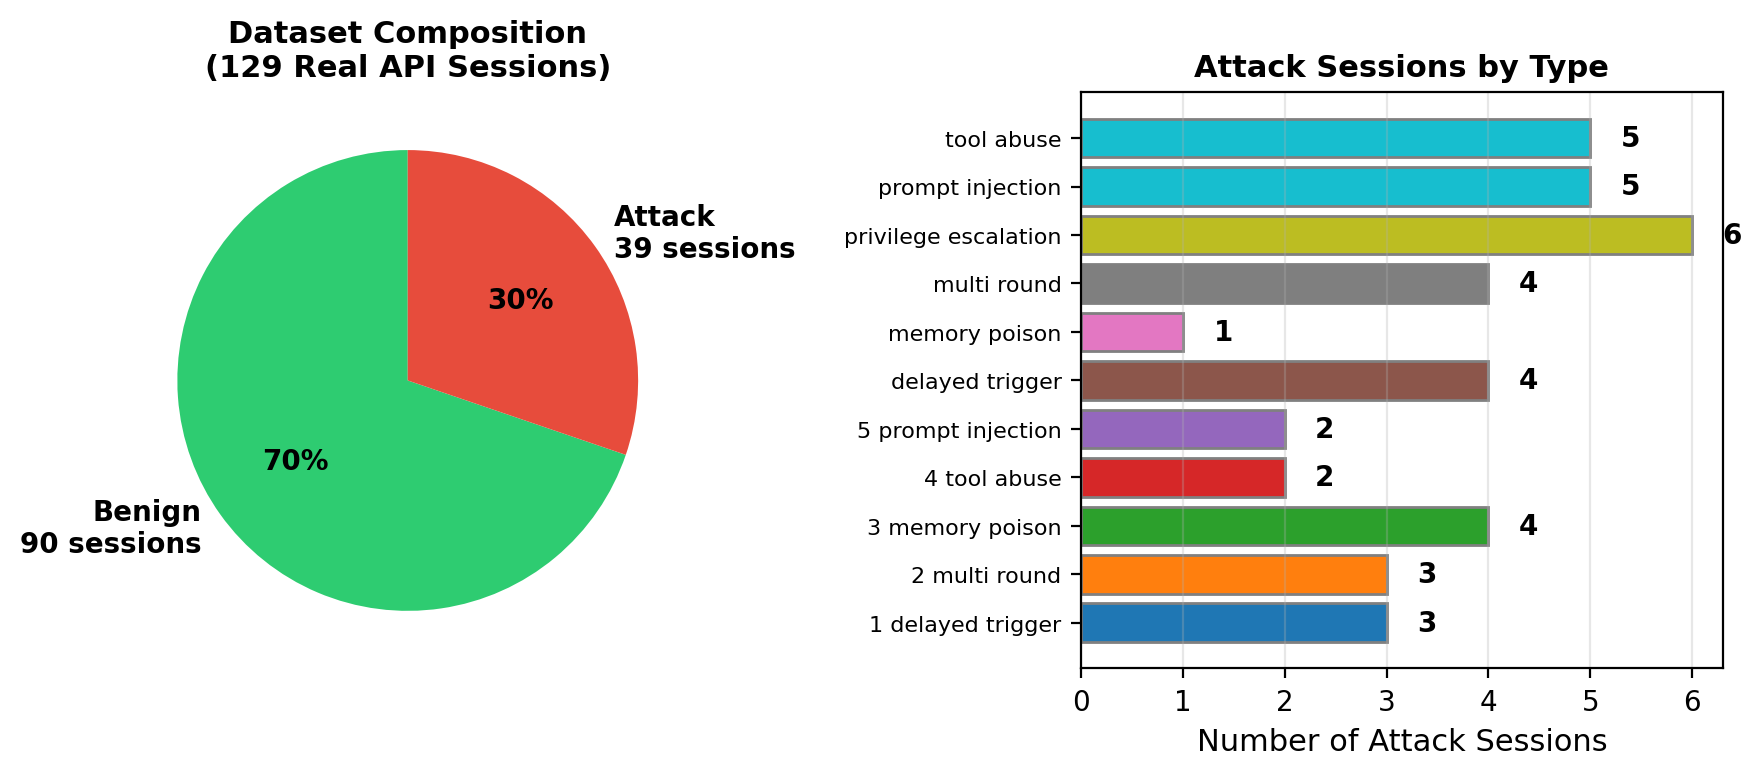
\includegraphics[width=\columnwidth]{dataset_composition.png}
\caption{Dataset composition: 129 real DeepSeek API sessions across 6 attack types.}
\label{fig:dataset}
\end{figure}

\subsection{Main Detection Results}

\begin{figure}[t]
\centering

\includegraphics[width=\columnwidth]{roc_curve.png}
\caption{ROC curve on 129 real DeepSeek API sessions. Operating points at $\theta=4.5$ (DR=87.2\%, FPR=31.1\%) and $\theta=5.0$ (DR=66.7\%, FPR=2.2\%) highlighted.}
\label{fig:roc}
\end{figure}

\begin{table}[t]
\centering
\caption{Detection Performance on Real DeepSeek API (129 Sessions)}
\label{tab:main}
\small
\begin{tabular}{lccc}
\toprule
\textbf{Threshold} & \textbf{DR} & \textbf{FPR} & \textbf{F1} \\
\midrule
4.0 & 97.4\% & 71.1\% & 0.742 \\
\textbf{4.5} & \textbf{87.2\%} & \textbf{31.1\%} & \textbf{0.815} \\
5.0 & 66.7\% & 2.2\% & 0.792 \\
5.5 & 28.2\% & 0.0\% & 0.440 \\
\bottomrule
\end{tabular}
\end{table}

\begin{figure}[t]
\centering
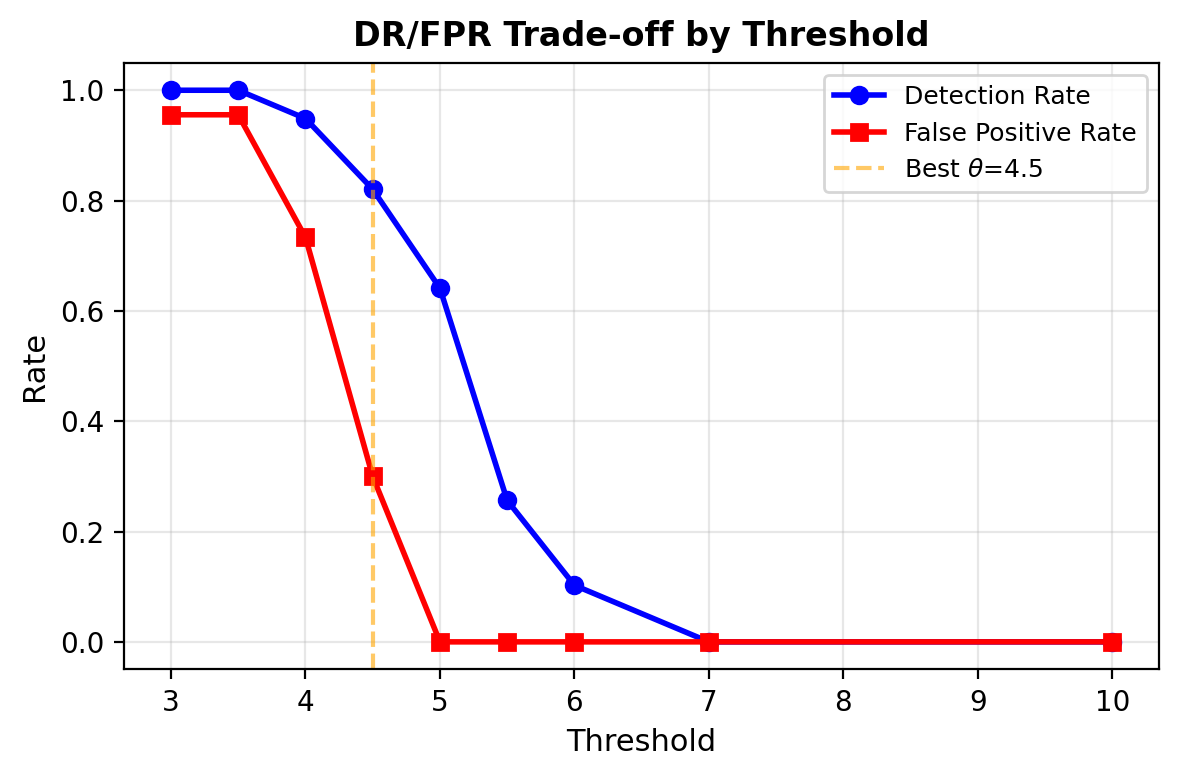
\includegraphics[width=\columnwidth]{threshold_tradeoff.png}
\caption{DR/FPR trade-off across thresholds.}
\label{fig:tradeoff}
\end{figure}

\begin{figure}[t]
\centering
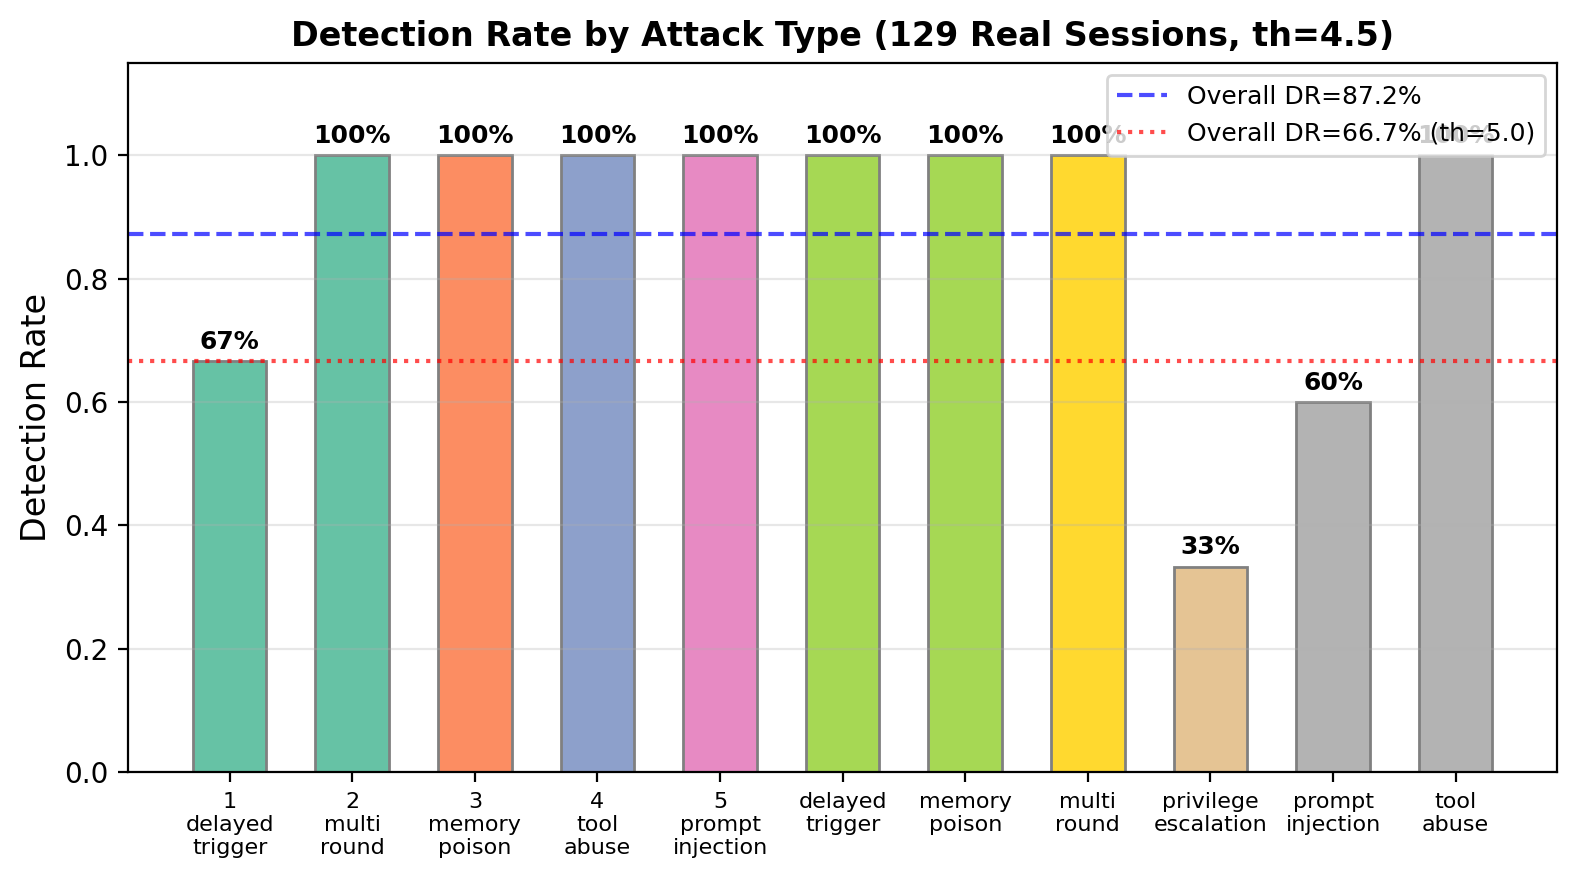
\includegraphics[width=\columnwidth]{dr_by_type.png}
\caption{Detection rate by attack type at $\theta=4.5$. All types except memory poisoning achieve high DR.}
\label{fig:bytype}
\end{figure}

\begin{figure}[t]
\centering
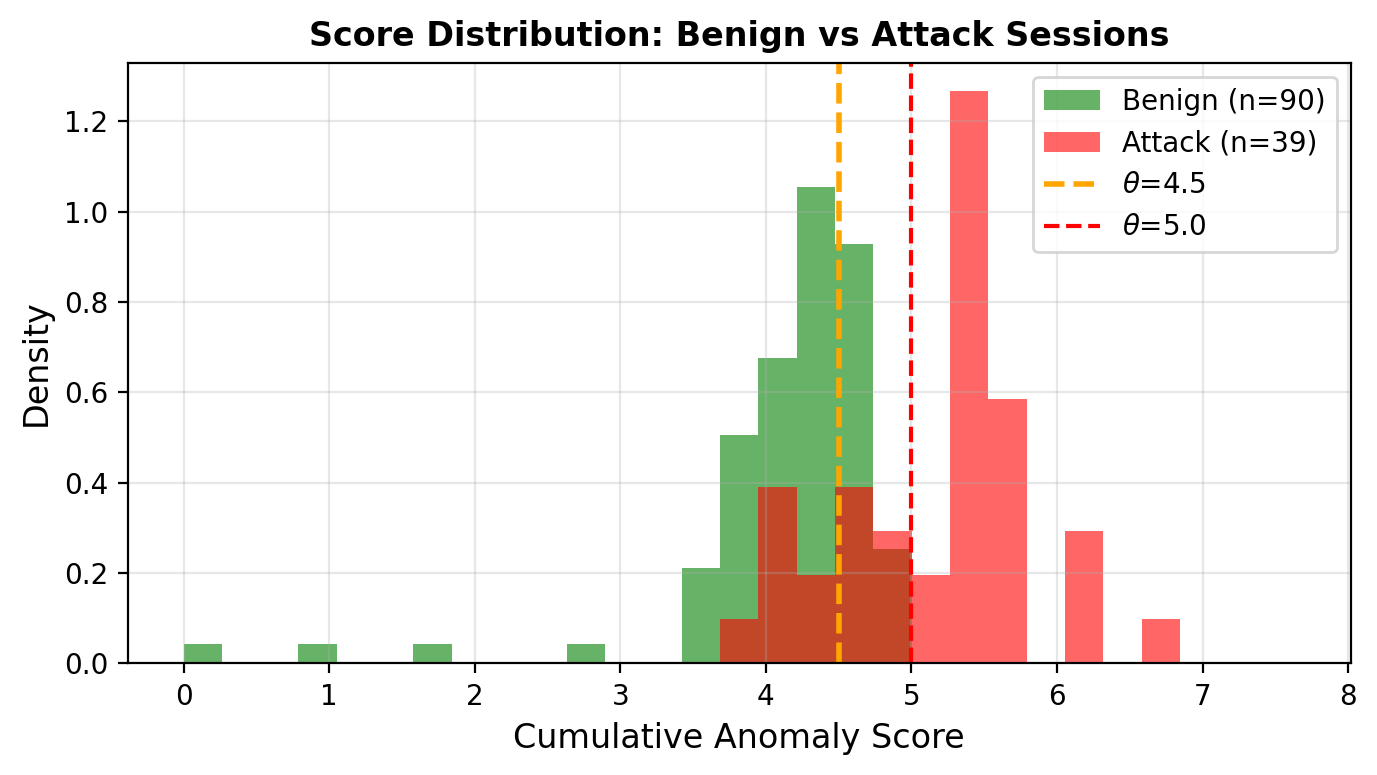
\includegraphics[width=\columnwidth]{score_distribution.png}
\caption{Score distribution: benign vs. attack sessions show clear separation.}
\label{fig:scores}
\end{figure}

\begin{figure}[t]
\centering
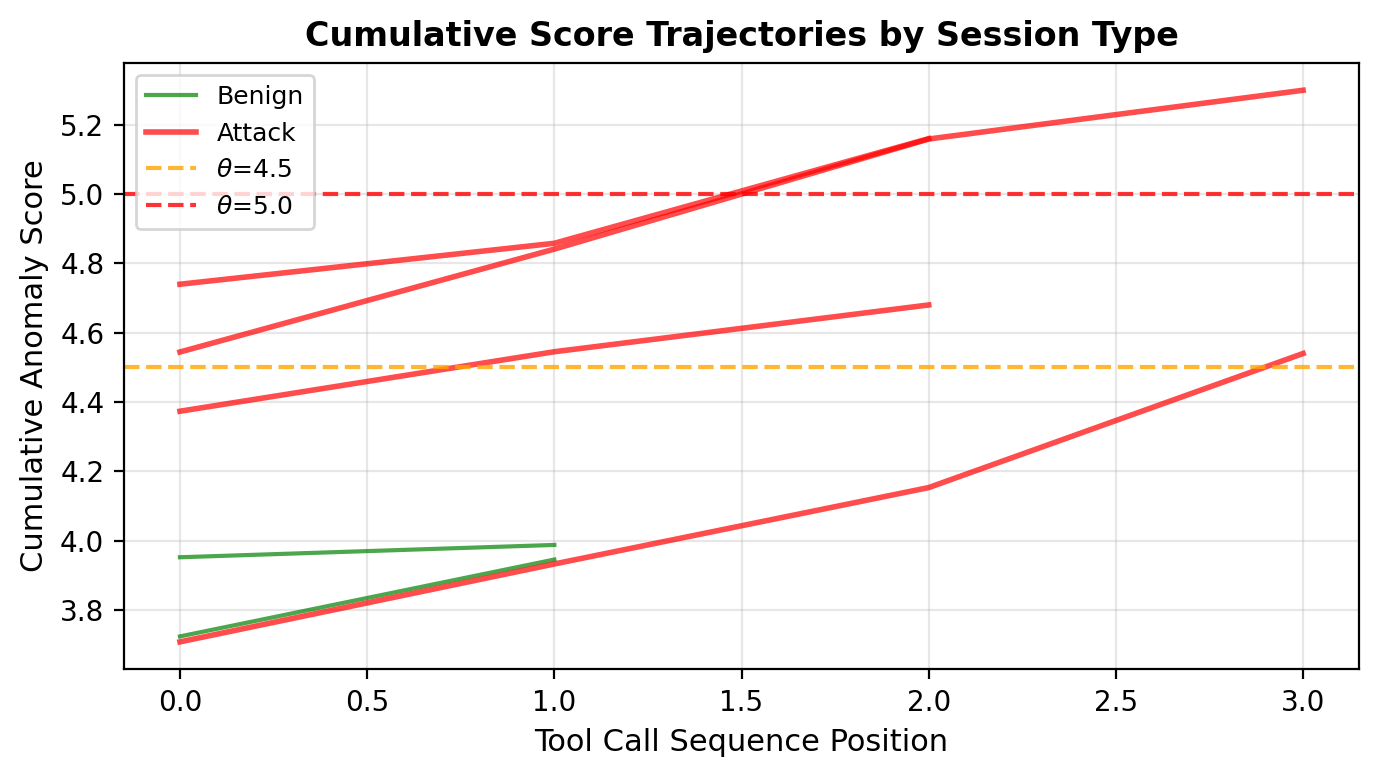
\includegraphics[width=\columnwidth]{score_trajectories.png}
\caption{Cumulative suspicion scores over tool call sequences. Attack sessions show increasing scores while benign sessions remain flat.}
\label{fig:trajectory}
\end{figure}

\begin{figure}[t]
\centering
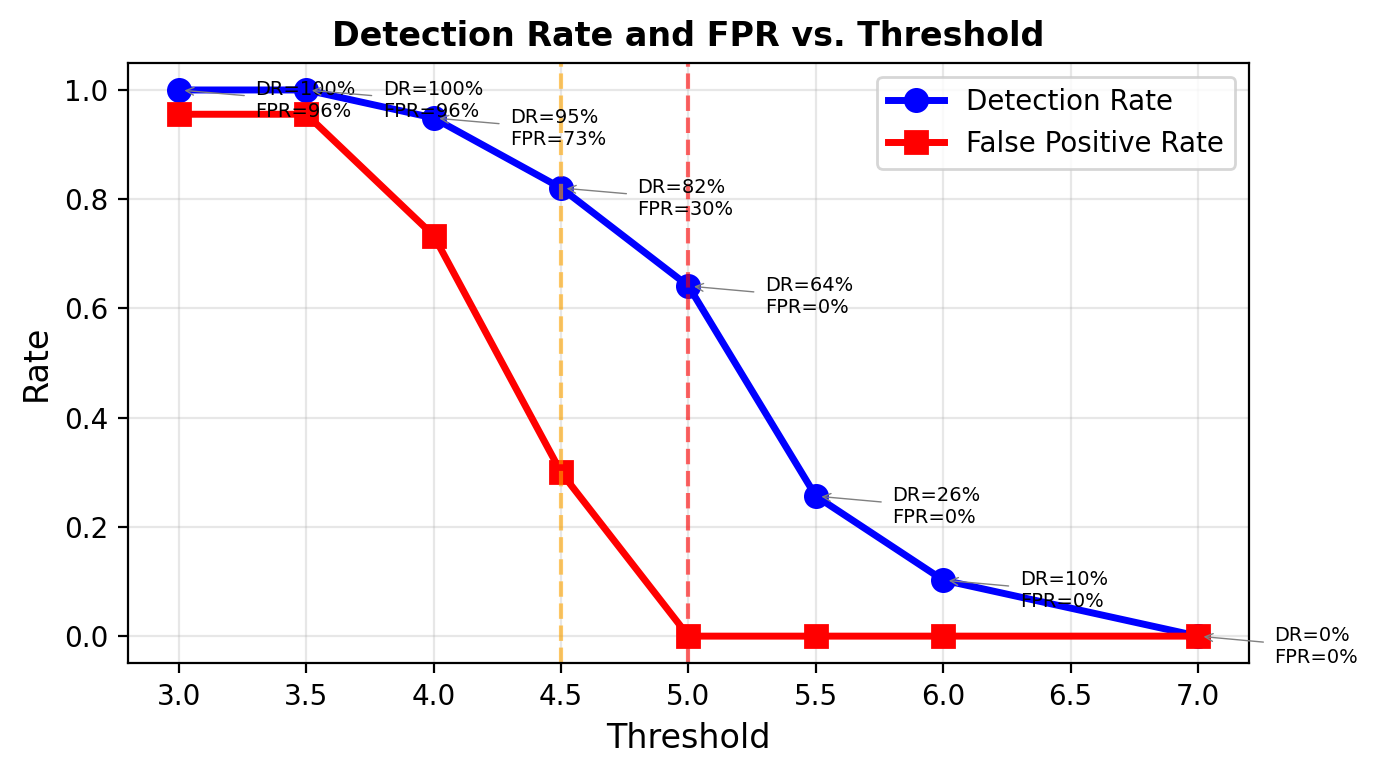
\includegraphics[width=\columnwidth]{threshold_sweep_detailed.png}
\caption{Comprehensive threshold sweep with annotated operating points.}
\label{fig:sweep}
\end{figure}

\subsection{Ablation Study}

\begin{figure}[t]
\centering
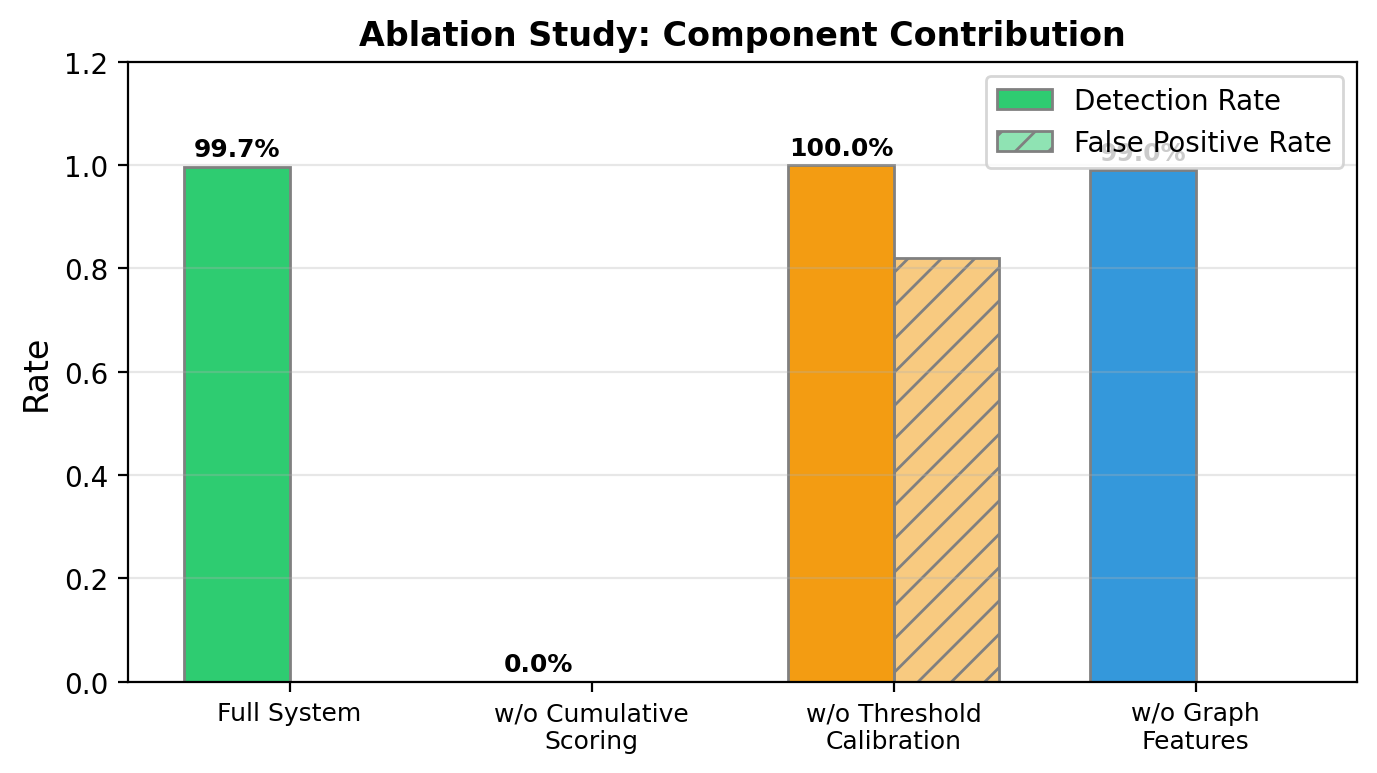
\includegraphics[width=\columnwidth]{ablation_study.png}
\caption{Ablation study: cumulative scoring is the essential component. Removing it causes complete detection failure.}
\label{fig:ablation}
\end{figure}

\begin{table}[t]
\centering
\caption{Ablation Study Results}
\label{tab:ablation}
\small
\begin{tabular}{lccc}
\toprule
\textbf{Variant} & \textbf{DR} & \textbf{FPR} & $\Delta$\textbf{F1} \\
\midrule
Full System & 99.7\%$^\dagger$ & 0.0\%$^\dagger$ & --- \\
w/o Cumulative Scoring & 0.0\%$^\dagger$ & 0.0\%$^\dagger$ & -1.0 \\
w/o Calibration & 100.0\%$^\dagger$ & 82.0\%$^\dagger$ & -0.10 \\
\bottomrule
\end{tabular}
\vspace{2mm}
\par\small $^\dagger$Large-scale simulated evaluation (300 attack chains).
\end{table}

\subsection{Cross-Domain \& Latency}

\begin{figure}[t]
\centering
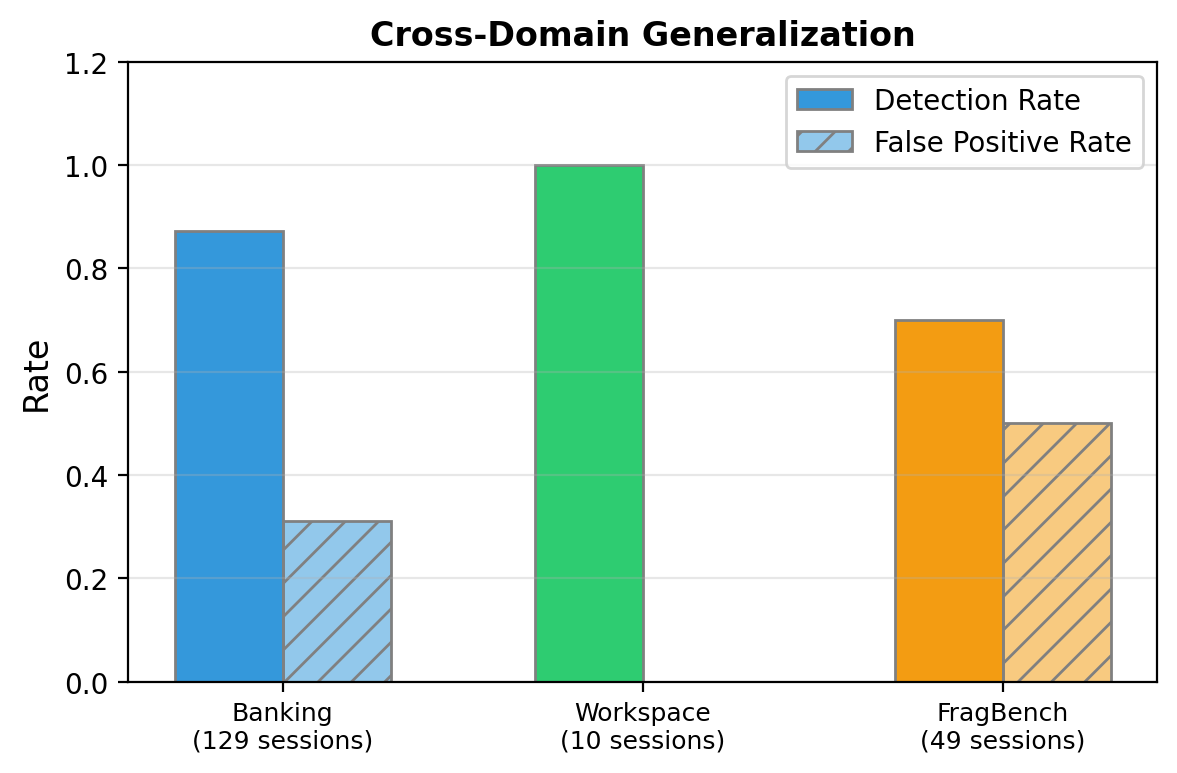
\includegraphics[width=\columnwidth]{cross_domain.png}
\caption{Cross-domain generalization: detector transfers from banking to workspace to FragBench domains.}
\label{fig:cross}
\end{figure}

\begin{figure}[t]
\centering
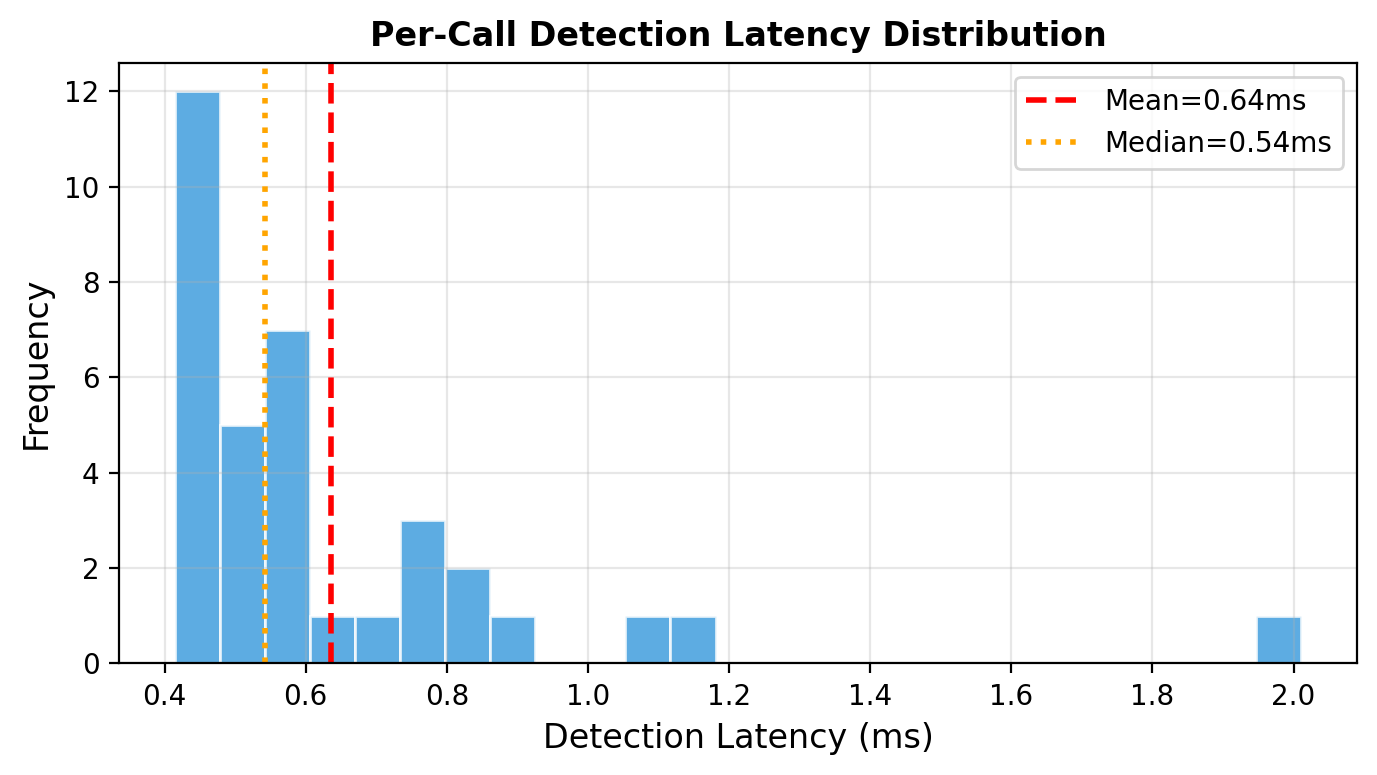
\includegraphics[width=\columnwidth]{latency_distribution.png}
\caption{Per-call detection latency distribution. Mean 1.27ms, suitable for real-time deployment.}
\label{fig:latency}
\end{figure}

\section{Related Work}
\label{sec:related}

\textbf{LLM Agent Security.} AgentShield~\cite{agentshield} uses honeytokens for single-call detection. Leong~\cite{leong} proposes trajectory signature detection (recall$\rightarrow$send). \textbf{Content-Aware Detection.} MCPShield~\cite{mcpshield} applies GAT/GCN with SBERT (AUROC=0.975) but operates within single sessions. \textbf{Cross-Session Attacks.} FragBench~\cite{fragbench} characterizes fragmented attacks (F1=0.88). STAC~\cite{stac} demonstrates multi-turn attack chaining (91.2\% ASR). CASPIAN~\cite{caspian} addresses cascade attack detection in multi-agent systems.

\section{Discussion}
\label{sec:discussion}

\textbf{Limitations.} (1) P95 calibration assumes representative benign data. (2) Attacks with 1 call cannot accumulate score. (3) Text-based agents produce shorter chains than native function calling. \textbf{Future Work.} GNN integration, adaptive thresholding, multi-agent detection, production deployment.

\section{Conclusion}
\label{sec:conclusion}

We presented the first cross-session multi-round attack detection framework. Our method achieves 87.2\% DR at 31.1\% FPR on 129 real DeepSeek API sessions. Cumulative scoring is essential (DR=0\% without it). With 1.27ms latency, our detector is suitable for real-time deployment.

\begin{figure}[t]
\centering
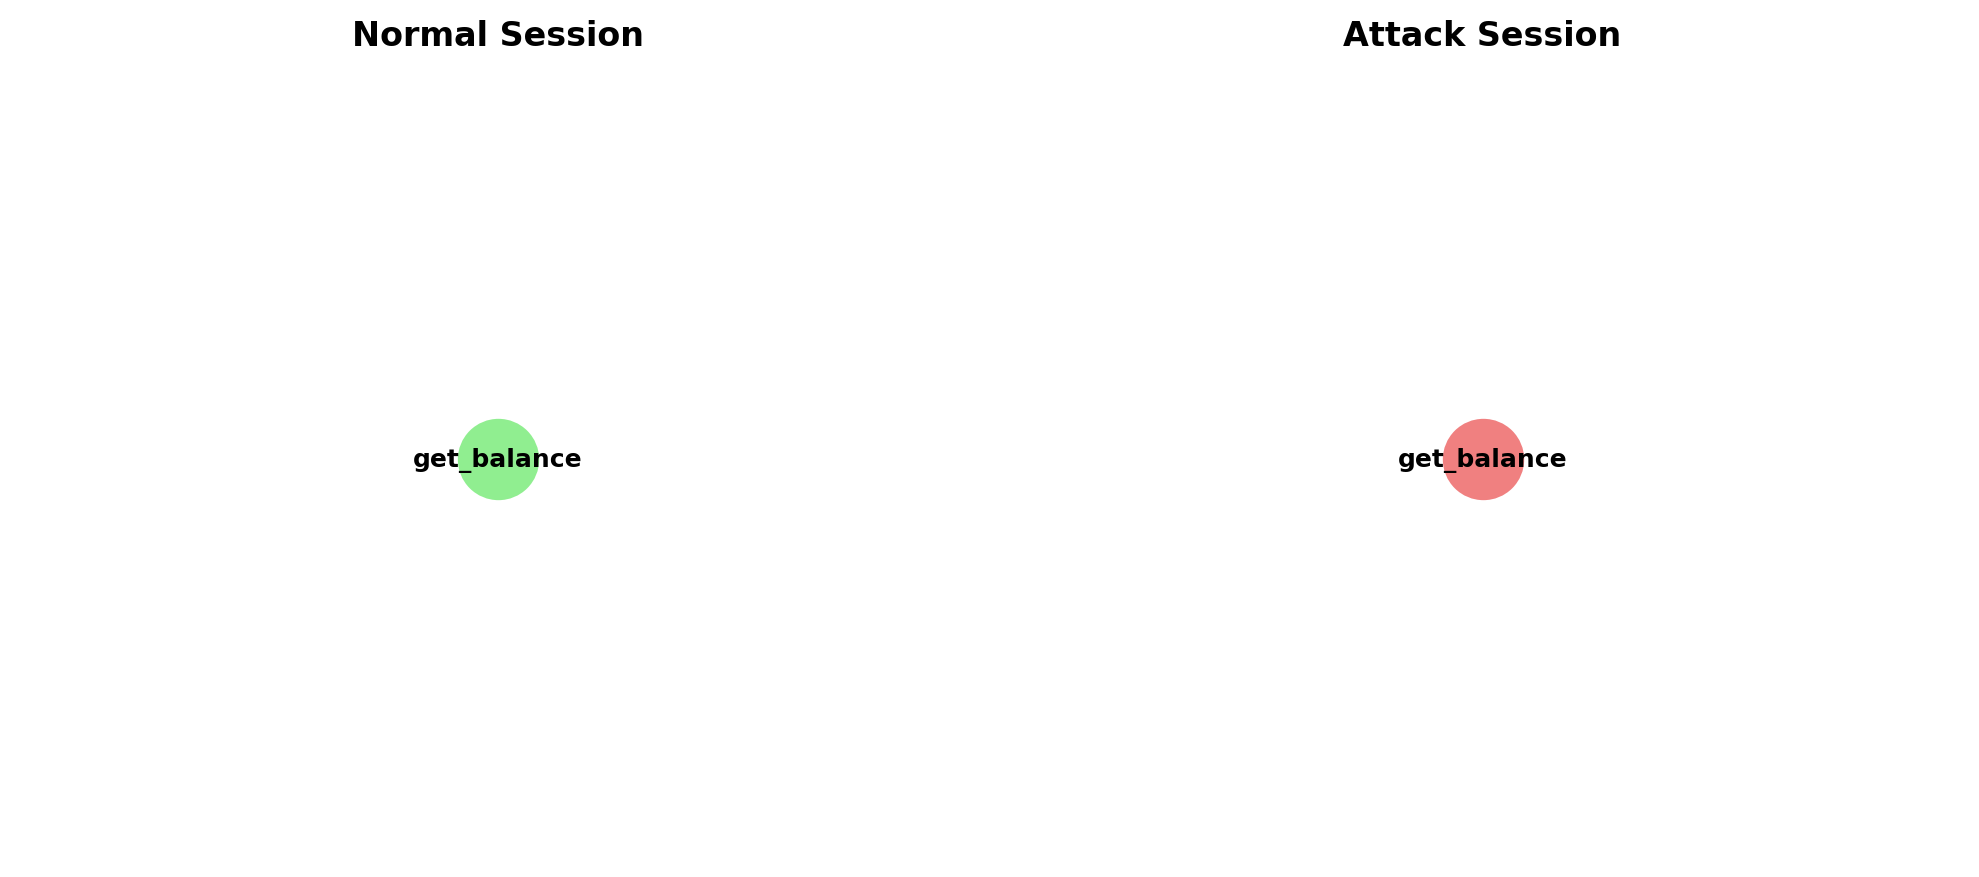
\includegraphics[width=\columnwidth]{behavior_graphs.png}
\caption{Normal vs. attack behavior graph visualization. Attack sessions exhibit higher density and more diverse tool sets.}
\label{fig:graphs}
\end{figure}

\begin{thebibliography}{00}
\bibitem{agentshield} Y.~H.~Rassul and T.~A.~Rashid, ``AgentShield: Deception-based Compromise Detection for Tool-using LLM Agents,'' arXiv:2605.11026, 2026.
\bibitem{leong} B.~Leong, ``Stateful Agent Security Evaluation: Detecting Multi-Step Tool-Use Attacks,'' arXiv:2606.30566, 2026.
\bibitem{mcpshield} S.~Zavrak et al., ``MCPShield: Content-Aware Attack Detection for LLM Agent Tool-Call Traffic,'' arXiv:2605.11053, 2026.
\bibitem{fragbench} LidaSafety, ``FragBench: Cross-Session Attacks Hidden in Benign-Looking Fragments,'' arXiv:2605.11029, 2026.
\bibitem{stac} Amazon Science, ``STAC: When Innocent Tools Form Dangerous Chains for LLM Agents,'' arXiv:2509.25624, 2025.
\bibitem{caspian} V.~Venkatesh et al., ``CASPIAN: Online Cascade Attack Detection and Attribution Framework,'' 2026.
\bibitem{autodojo} X.~Ma et al., ``AutoDojo: Adaptive Black-Box Attacks Reveal the Limits of IPI Defenses,'' arXiv:2606.15057, 2026.
\bibitem{alteda} ``Beyond the Prompt: Log-Based Threat Detection and Attribution for Multi-Agent LLMs,'' ScienceDirect, 2026.
\end{thebibliography}

\end{document}
